%% • The introduction must be dynamite. 
%% – The reader forms an oppinion of the work right from the start... 
%% • The introduction is an extension of the abstract. 
%% • Should be easy to read and understand 
%% • Should make it easy for anyone to tell
%% – What your paper is about 
%%   – What problem it solves
%%   – Why the problem and solution is interesting and relevant (motivation and context). Is it a long- outstanding problem?
%%   – What is new in your paper and how (much) does it improve on the strongest alternatives/previous work (include a few of the most relevant references here).

%% • Start the introduction with the motivation. Think in large contexts and don’t be afraid to be a poet.
%% • All implications, contributions and keypoints of your work must be included here.
%% • Make it very clear how your work will impact the future of Realistic image generation (will people use it?).
%% • If your work is pioneering, s-p-e-l-l i-t o-u-t.
%% • Briefly make it clear how you evaluate your method in the Results section.
%% • Make sure to explain where your method applies and where it does not apply (limitations).


\chapter{Introduction}

\chapterquote{Focus is a matter of deciding what things you're not
  going to do.}{John Carmack}

%% \section{Old intro}

%% \textit{Rendering} is the process of converting a description of a
%% scene into an image and is what lies at the heart of \textit{computer
%%   graphics}.

%% Several techniques exist that allows computers to perform this
%% conversion. When real-time rendering is needed, the most commonly used
%% technique is \textit{rasterization}, in which vertex attrbiutes of
%% geometric shapes are mapped onto a raster\footnote{A flat, 2D grid.}
%% and subsequently \textit{shaded}. Due to the popularity of this
%% technique in computer games, hardware accelerated rasterizers have
%% become quite powerful over the last decade and are now able to process
%% millions of geometric primitives pr. second. However, certain aspects
%% of rendering are not easily solved by rasterization.
%% \textit{Reflection} and \textit{refraction} effects on non-flat
%% surfaces are notoriously hard to recreate, due to the divergence of
%% individual light rays at these points, and must instead be
%% approximated. Reflection by an object is usually approximated by
%% \textit{environment mapping}, as can be seen on
%% \reffig{fig:cubemap}. The problem with this approch is that the scene
%% will have to be rendered an additional 6 times for each frame.

%% An alternative to rasterization is presented by \textit{ray casting}
%% or \textit{ray tracing}. In ray tracing, each individual pixel is
%% shaded by tracing one or more \textit{primary rays} ``cast'' from the
%% camera into the world and observing which primitive they
%% intersect. Reflection and refraction are easily created by spawning a
%% new ray at the intersection point and then tracing it. In contrast to
%% rasterization this provides a much more correct result, easily allows
%% for multiple \textit{reflection rays} and as we shall see in section
%% TODO at a much better lower cost increase pr. frame. Shadows are also
%% easily created using ray tracing. Hard edged shadows can be created by
%% tracing a \textit{shadow ray} from an intersection point towards a
%% lightsource. If the shadow ray intersects another part of the world
%% before it reaches the lightsource, then the intersection point must be
%% placed in shadow and does not receive any illumination from the
%% lightsource. Using advanced lighting algorithms such as \textit{photon
%%   mapping}, which incorporates ray tracing for light transportation,
%% lighting from reflective surfaces, color bleeding and even correct
%% caustics can be simulated.


%% Nevertheless, the photorealistic images rendered by ray tracers does
%% come at a high computational cost, which is why ray tracing is mostly
%% used for \textit{offline rendering}, for example for special effects in
%% movies or high quality images.

%% % Due to increase on computing power, we're getting closer and closer
%% % to seeing real-time ray tracing and it's lighting in
%% % applications. Bla bla rewrite!

%% % The evergrowing interest in photorealistic rendering and the
%% % complexity of the scenes rendered.

%% But, due to the everincreasing computational power and continued
%% research into \textit{global illumination acceleration techniques},
%% the physically correct image quality obtainable though ray tracing is
%% becoming more and more alluring to designers of real-time graphical
%% applications, especially if correct reflection or refraction is
%% needed.

%% % Why global illumination vs local illumination used in most
%% % rasterizers. Ray tracing can produce more correct images, and it
%% % scales $O(N log M)$, whereas rasterizers scale O(NM) or O(N+M).

%% \fxfatal{time complexity?}

%% % Why use the GU? Offloading. The CPU can do a lot of other things
%% % while the GPU crunch away at those KD trees. Om nom nom nom
%% % nom.... Games already make heavy use of the CPU for game logics,
%% % networking and AI, they need to offload graphics to the another
%% % processing unit.

%% In this thesis I will be combining the rendering quality of ray
%% tracing with the computational power of modern
%% \textit{GPGPU}'s\footnote{General Purpose Graphics Processing
%%   Units.}. This requires that the algorithms presented exploit the
%% massively dataparallel nature of the graphics card, requiring
%% thousands of threads for each GPGPU program. This subject will be
%% discussed in \refchapter{chp:GPGPU}

%% There are several good reasons for using GPGPU's for ray tracing. Each
%% ray can be traced independently and in parallel with all the other
%% rays. Even at a resolution of 512x512, 262144 primary rays are
%% generated, resulting in more than enough threads to potentionally
%% utilize all of the GPGPU's multiprocessors. In the case of computer
%% games, the CPU is already heavily occupied with \textit{game logic},
%% \textit{networking}, \textit{AI}\footnote{Artificial Intelligence},
%% and more to also handle rendering, in which case offloading to an
%% otherwise idle GPGPU only makes sense. Recent advances in GPGPU ray
%% tracing have also shown performance comparable to CPU
%% implementations\citebook{1230129}\citebook{popov:07:GPURT}, meaning
%% the choice of architecture can now be based purely on where most
%% performance will be available.

%% Recent advances in acceleration structure creation have allowed them
%% to be created equally fast on the CPU and
%% GPGPU\citebook{1409079}. Therefore, as with ray tracing, this thesis
%% will focus on a GPGPU implementation, to reduce the workload of the
%% CPU. Keeping the entire workload on the graphics card has the added
%% benefit of minimizing datatransfers over the bus.

%% % In this thesis I present an exhaustive ray tracer and compared it to
%% % a basic non optimized ray tracer traversing a KD-tree, to emphasize
%% % the importance of datastructures, even on the GPU.

%% % importance of efficient datastructures, several datastructures have
%% % been used for ray tracing (BVH, kd-trees, octrees, bla bla...) Some
%% % are good for bla, others blank

%% % Reference the 'good' kd tree double speed up and how it doesn't say
%% % anything about the extra time spend on these good tree.

%% % can be done by parallising the evaluation of the approximate cost of
%% % each node

%% % \textit{Surface Area Heuristic}, $SAH$, 

%% % and creation of nodes at lower tree levels

%% % Still not easily paralisable, requires lots of reduction kernels,
%% % which do not utilize the GPU fully. Also individual node splitting
%% % costs can leave 31 threads in a warp waiting for the last one to
%% % finish.


% Motivation

\textit{Rendering} is the process of converting a description of a
scene into an image and is what lies at the heart of \textit{computer
  graphics}. The ability to render complex scenes realistically or
distinctly is vital in several areas; computer games, movies and even
medical imaging.


% Rasterization and cubemapping

When real-time rendering is needed the technique of choice for the
last one and a half decade has been \textit{rasterization}. In
rasterization a geometric primitives vertex attributes, such as their
position, normal and color, is mapped into a
\textit{raster}\footnote{A flat, 2D grid.} and its color is
calculated. This technique is so popular in the game industry that
processing units where created specifically for rasterization, the
\textit{Graphics Processing Unit} or \textit{GPU} for short. Due to
the industry's ever increasing demand for more detailed models and
effects, the GPU's have seen a massive increase in both computational
power and throughput over the last decade, as evidenced by
\reffig{fig:gflops}. Unfortunatly, even with all this power certain
aspects of rendering are still not easily solved by
rasterization. \textit{Reflection} and \textit{refraction} effects on
non-flat surfaces are notoriously hard to recreate, due to the
divergence of spatially close light- and reflection rays at the points
in which they intersect the geometry. Reflections of complex objects
can be approximated by \textit{environment mapping} or \textit{cube
  mapping}, a short describtion can be found on
\reffig{fig:cubemap}. The trouble with cubemapping is that the scene
will have to be rendered another 6 times for each cubemap, increasing
the cost of rendering by up to 6 times. Another short coming of
cubemapping is that it doesn't support \textit{self reflection}, since
it is only the surrounding environment that is rendered onto the map.

\begin{figure}
  \centering
  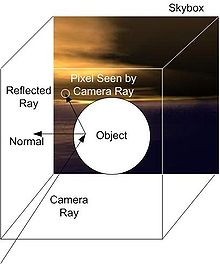
\includegraphics{Cube_mapped_reflection_example}
  
  \vspace{3mm}
  \parbox{9.5cm}{\caption[Cube mapping visualized.]{A visualization of
      cube mapping. The environment is rendered onto the sides of the
      cube and then mapped onto the sphere. The mapping is performed
      by using the calculated reflection vector as a texture
      coordinate.\\Image from
      http://en.wikipedia.org/wiki/Reflection\_mapping}\label{fig:cubemap}}
\end{figure}

% Ray tracing and comparing it to rasterization

Another technique for rendering is \textit{ray tracing}, which
eloquently solves reflection and refraction by tracing rays from the
eye and into the scene, spawning and tracing new reflection and
refraction rays as needed when geometry is intersected. A comparisson
of cube mapping and ray tracing of a reflecting stanford dragon can be
seen in \reffig{fig:reflectingDragons}. Notice how the ray traced
dragons backside reflects its neck, while the cubemapped version only
reflects the surrounding box. Advanced lighting techniques that
produces photorealistic images are also based on ray tracin. One such
technique is \textit{photon mapping}, which can accurately reproduce
the effects of lighting from reflective surfaces, caustics and color
bleeding.


% High cost used to make it unattractive for interactive scenes

The increased realisme that can be achieved with ray tracing does come
at a high computational cost, however, which has previously made it
unattractive for interactive applications or dynamic
scenes. Nonetheless, the recent increase in computational power
coupled with research into the area of \textit{interactive ray
  tracing} have yielded some incredible results.

\begin{figure}
  \centering
  \subfloat[A cubemapped reflecting dragon.]{
    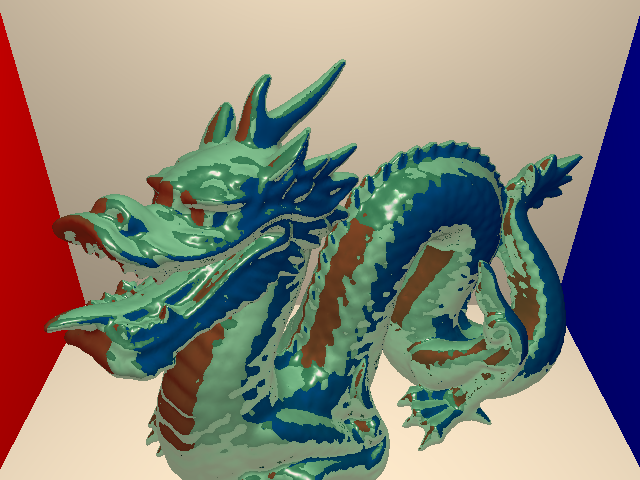
\includegraphics[width=7cm]{cubemappedDragon}
    \label{fig:cubeDragon}
  }
  \hspace{10pt}
  \subfloat[A ray traced reflecting dragon. Notice the self reflection
    on the back and inside the mouth.]{
    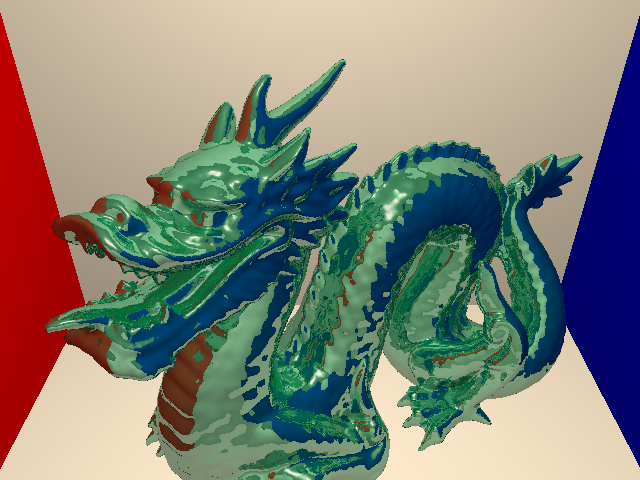
\includegraphics[width=7cm]{semiReflectingDragon}
    \label{fig:rayReflectingDragon}
  }
  \caption[Cubemapping vs raytracing for reflections.]{An example of
    the difference between using cubemapping or raytracing for
    reflections.}
  \label{fig:reflectingDragons}
\end{figure}


% What I will show, doing it dynamically, which is interesting for
% games and movie development

In this thesis I will examine \textit{ray tracing of dynamic scenes},
which could become an interesting alternative to rasterization in the
gaming industri and certainly is interesting for 3D artists working on
large screen movie productions, where ray tracing is already used for
\textit{CGI}\footnote{Computer-generated Imagery} effects and the
artists need to quickly be able to rearrange the scene.


% We need Acceleration stuctures for ray tracing to achieve this

To speed up ray tracing, several data structures have been
developed. This thesis will focus on the \textit{kd-tree}, a
\textit{binary space partition} tree which recursively subdivides
$k$-dimensional geometry by splitting it with \textit{axis aligned
  splitting planes}. One such subdivision can be seen on
\reffig{fig:binarySplit}. A kd-tree's quality is related to the choice
of splitting planes and a lot of computational power can go into
finding optimal splitting planes, as every possible useful splitting
plane must be considered. A high quality kd-tree will place spatially
close geometric primitives close together in the tree. This is the
topic of \refsection{sec:splittingPlane}. In order to facilitate
dynamic scenes, the data structure must also be
dynamic. Uunfortunatly, in the case of kd-trees this means completely
rebuilding it. Due to this the algorithm for creating the kd-tree
needs to be very fast, and might have to sacrifice tree quality for
speed. It is this compromise that will be studied in this theses.



% Why do it on the GPU, yes why indeed? Leaves the CPU free to do
% other things than rendering.

As observed above, the GPU's have grown quite powerful over the last
decade, and since the introduction of programmable GPU's and
NVIDIA's \textit{CUDA}\footnote{Compute Unified Device Architecture.}
framework, many algorithms have been succesfully ported to utilize the
resources of the GPU. I will be doing the same in this thesis and use
the GPU to accelerate the creation of data structures and ray tracing
them. The most compelling reason to do this, is that it leaves the CPU
free to handle other aspects of a graphics application, such as for
instance game logic and networking in a computer game.



\section{Goals}

In this thesis the goal is not to produce images of photorealistic
quality, or create an interactive ray tracer for dynamic
scenes \footnote{This goal in itself can trivially be achieved by
  reducing the complexity of the scene or lowering the resolution.}
Instead this thesis will explorer ray tracing acceleration structures,
specifically the kd-tree, and it's impact on ray tracing efficiency
for dynamic scenes.

There are 3 ways to optimize ray tracing with respect to dynamic
scenes. 

\begin{enumerate}
  \item \textbf{Create a faster ray tracer -} Several optimizations
    exists that improve the speed of a ray tracer independently of the
    underlying acceleration stucture. These will be the focus of
    \refsection{sec:hierarchicalTraversal}.
  \item \textbf{Building a higher quality acceleration structure -} An
    acceleration structure of higher quality can reduce the time it
    takes the ray tracer to find the nearest intersecting point
    between a ray and a primitive. Algorithms for producing kd-tree's
    of different quality is the topic of
    \refsection{sec:splittingPlane}.
  \item \textbf{Build the acceleration structure faster -} In a
    dynamic scene, the acceleration structure may need to be rebuild
    for each frame. Being able to rebuild it fast is therefore
    crucial. One way to ensure a faster reconstruction is by reducing
    the time spend deciding where to place the splitting plane, which
    can result in trees of lower quality.
\end{enumerate}

The main topic in this thesis is the relationship between tree quality
and construction speed and if the overall time it takes to ray trace a
scene can be improved by sacrificing tree quality for speed.

During this thesis I will also look at the usefullness of using an
acceleration structure, given the added overhead of keeping it updated
and the GPU's difficulty processing neighbouring threads with
different execution paths, as those of threads choosing different
paths through a tree. These problems will be detailed in
\refsection{sec:threadHierarchy}. An exhaustive ray tracer, which will
intersect every ray with every triangle and thus has a more
straightforward execution path, is implemented to motivate the use of
a hierachical datatstructure.

The kd-tree implementation used for accelerating ray tracing will be
based on the implementation described by \zhou.  Improvements to the
quality of the tree include which algorithm to use when determining
where to split the scene and \textit{empty space maximization}, which
facilitates an early out option for the ray tracer.

\fixme{Uddyb hvorfor der skal splittes, nævn splitting plane}

The thesis will also look at alternate ways of assigning triangles to
nodes on each side of the splitting planes. The most common technique
is \textit{triangle splitting}. I propose and investigate 2 different
approaches, in which the triangle is not split into new triangles, but
instead merely assigned to both nodes upon overlapping, which should
result in less triangles being created due to splits and thus a
smaller kd-tree.

Strategies that optimize the KD-tree will be evaluated based on the
time added to the kd-tree creation phase, and the time saved in the
ray tracing phase.

To give a fair comparison of the time spend ray tracing and the time
spend building the data structure, I will need to create an optimized
ray tracer. Optimizing the ray tracer for this comparison is
important, since the optimized implementation is up to 80\% faster
than the basic implementation, with no added cost or logic to the
kd-tree creation phase. Optimizations to the ray tracer will be
inspired by the work done by \horn , but also include investigation of
optimal ray/triangle intersection algorithms, an improvement inspired
by empty space maximization during kd-tree creation and simply
structuring the rays in a manner that favors SIMD execution.

Ray tracing optimizations will simply be evaluated based on time saved
during ray tracing. Optimizations will be based on improving the
worst case scenarios, i.e. long rays shooting towards the center of
the scene.

\section{Overview}

The thesis is structured as follows:

% Previous work

The next section details previous work in the area of ray tracing and
kd-tree construction. This includes a brief history of when ray
tracing was introduced, aswell as key points in time for different
acceleration structures. The last part of this section will focus on
kd-trees and ray tracing on graphics hardware. Changes in this thesis
compared to previous work in the area are also outlined in this
section.

% Understanding the GPGPU

A chapter will then introduce the GPGPU\footnote{General Purpose
  Graphics Processor Unit. A programable graphics processor.}
architecture. Here I will describe CUDA's thread and memory model. I
will then go on to describe a new primitive as proposed by Sengupta et
al.\citebook{Sengupta:2007}, which will be helpful for performing
scattering and compaction on graphics hardware. Finally this
section will focus on optimization techniques specific to CUDA. These
will be applied incrementally in a case study of a global minima
algorithm.

% kd-trees

\refchapter{chp:kdTrees} is then devoted to discussing kd-trees. The
first part of this section deals with the general kd-tree construction
algorith. Here I will present several algorithms for choosing the
splitting plane and discuss 3 different algorithms for associating
triangles with child nodes. The second part of the section deals with
the actual implementation of kd-trees on a GPU.

% raytracing

Having introduced kd-trees, the next chapter will deal with the
algorithms for traversing such trees and ray tracing the scene. Here
several optimizations to a basic raytracer will be discussed and
incrementally added to the ray tracer. First though, an exhaustive ray
tracer is presented and will be used in the Results chapter to
motivate the use of hierarchical data structures on the GPGPU. This
section also includes a discussion of 2 triangle intersection
algorithms with respect to performance on the GPGPU. The section ends
with a brief discussion of how colors and reflection/refraction
are calculated.

% Results

% Conclusion

% Future work
